\section{Proceso iterativo}

El algoritmo propuesto posee un proceso iterativo que se repite hasta satisfacer una cantidad de iteraciones o generaciones dadas por el parámetro \generaciones. A continuación se detallarán los pasos realizados en cada una de estas generaciones.

\subsection{Cálculo de aptitud}

Cada elemento $p$ de la población $P$ es evaluado mediante una función de aptitud para determinar si es mejor o peor que otras soluciones. Esta función $f_{apt}$ está dada por la ecuación \eqref{eq:fitness}.

\begin{equation}
\label{eq:fitness}
f_{apt}(p) = \alp \cdot \tilde{FO}_1(p) + \bet \cdot \tilde{FO}_2(p)
\end{equation}

Para determinar la aptitud de un elemento $p$, ésta se deberá evaluar en las funciones objetivo $FO_1$ y $FO_2$ dadas por las ecuaciones \eqref{eq:fo1} y \eqref{eq:fo2}, respectivamente. Dado que el orden de magnitud de las funciones objetivo es distinto, cada valor será normalizado por una cota inferior conocida para cada instancia. Así, se determinarán las magnitudes $\tilde{FO}_1$ y $\tilde{FO}_2$, según lo mostrado en las Ecuaciones \eqref{eq:lb1} y \eqref{eq:lb2}.

\begin{equation}
\label{eq:lb1}
\tilde{FO}_1(p) = \frac{FO_1(p)}{LB_{FO_1}}
\end{equation}

\begin{equation}
\label{eq:lb2}
\tilde{FO}_2(p) = \frac{FO_2(p)}{LB_{FO_2}}
\end{equation}

Finalmente, la aptitud de $p$ está dada por una poderación de $\tilde{FO}_1$ y $\tilde{FO}_2$, utilizando los parámetros \alp{} y \bet. La función de aptitud entregará valores entre 0 y 1, siendo el valor 1 la mejor aptitud posible.

\subsection{Eliminación de soluciones dominadas}

El algoritmo inmune trabaja sobre soluciones factibles no dominadas. Al inicio de cada iteración, posteriormente al proceso de determinar la aptitud de las soluciones, se eliminan aquellas soluciones dominadas. Esto es, para realizar la transformación de soluciones que estén directamente en el frente de Pareto, con la intención de mejorarlas.

\subsection{Selección de soluciones}

Del conjunto de soluciones factibles no dominadas, se escoge un porcentaje de ellas para generar un conjunto de clones $C$. Las soluciones del conjunto $P$ son ordenadas de acuerdo a su aptitud en orden ascendente, y luego las primeras $mp$ soluciones se clonan de manera aleatoria en el conjunto $C$ hasta completar el tamaño \clonsize. La cantidad $mp$ es determinada utilizando el parámetro \pmejores{} como se muestra en la Ecuación \eqref{eq:mp}:

\begin{equation}
\label{eq:mp}
mp = \ceil*{|P| \cdot \pmejores}
\end{equation}

La cantidad $mp$ se detemina multiplicando la cardinalidad del conjunto $P$ por el parámetro \pmejores. A esta operación se le aplica la función techo para aproximar al entero superior.

\subsection{Operadores de transformación}

Los operadores de transformación utilizados en este algoritmo consisten en tres operadores de mutación, diseñados para generar cambios distintos en las soluciones con la esperanza de mejorar la función de aptitud de los anticuerpos. Los operadores trabajan generando un movimiento sobre una ruta de una solución. Estos operadores son agregar un paradero a una ruta, eliminar un paradero de una ruta y reordenar una ruta mediante un punto de corte.

\begin{enumerate}
\item \textbf{Agregar una ruta}: Considerando una ruta $r$ con $n$ paraderos ordenados: $bs_1, bs_2, \ldots, bs_n$. Este operador busca un vecino del paradero $bs_n$ y le agrega un nuevo paradero $bs_{n+1}$ al final de la ruta, dejando la ruta con $n+1$ paraderos ordenados. Este operador es factible de realizar en gran parte de los casos, exceptuando las rutas que tienen el máximo de paraderos permitidos. La Figura \ref{fig:mut1} muestra un ejemplo con $n=6$.

\begin{figure}[!htb]
\begin{center}
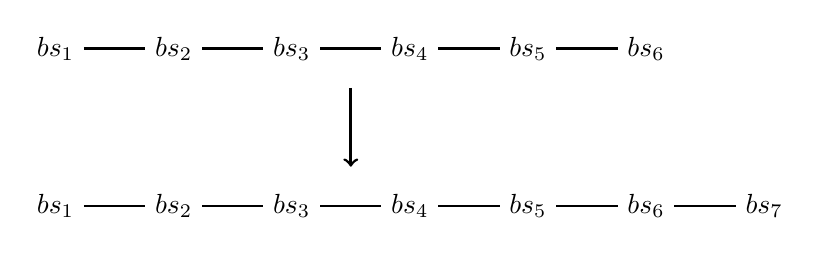
\begin{tikzpicture}
\node(1) at (0.0,0) {$bs_1$};
\node(2) at (1.5,0) {$bs_2$};
\node(3) at (3.0,0) {$bs_3$};
\node(4) at (4.5,0) {$bs_4$};
\node(5) at (6.0,0) {$bs_5$};
\node(6) at (7.5,0) {$bs_6$};

\draw[line width=1pt] (1) -- (2) -- (3) -- (4) -- (5) -- (6);

\draw[->,line width=1pt] (3.75,-0.5) -- (3.75,-1.5);

\node(1n) at (0.0,-2) {$bs_1$};
\node(2n) at (1.5,-2) {$bs_2$};
\node(3n) at (3.0,-2) {$bs_3$};
\node(4n) at (4.5,-2) {$bs_4$};
\node(5n) at (6.0,-2) {$bs_5$};
\node(6n) at (7.5,-2) {$bs_6$};
\node(7n) at (9.0,-2) {$bs_7$};

\draw[line width=1pt] (1n) -- (2n) -- (3n) -- (4n) -- (5n) -- (6n) -- (7n);

\end{tikzpicture}
\end{center}
\caption{Adición de un paradero al final de una ruta de 6 paraderos.}
\label{fig:mut1}
\end{figure}

\item \textbf{Eliminar una ruta}: Considerando una ruta $r$ con $n$ paraderos ordenados: $bs_1, bs_2, \ldots, bs_n$. Este operador elimina el último paradero $bs_n$, dejando la ruta con $n-1$ paraderos ordenados. Este operador es factible de realizar en gran parte de los casos, exceptuando las rutas que tienen el mínimo de paraderos permitidos. La Figura \ref{fig:mut2} muestra un ejemplo con $n=6$.

\begin{figure}[!htb]
\begin{center}
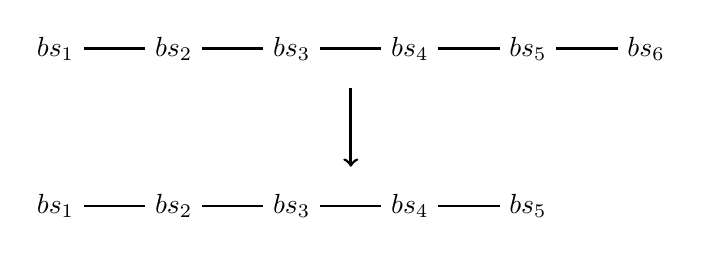
\begin{tikzpicture}
\node(1) at (0.0,0) {$bs_1$};
\node(2) at (1.5,0) {$bs_2$};
\node(3) at (3.0,0) {$bs_3$};
\node(4) at (4.5,0) {$bs_4$};
\node(5) at (6.0,0) {$bs_5$};
\node(6) at (7.5,0) {$bs_6$};

\draw[line width=1pt] (1) -- (2) -- (3) -- (4) -- (5) -- (6);

\draw[->,line width=1pt] (3.75,-0.5) -- (3.75,-1.5);

\node(1n) at (0.0,-2) {$bs_1$};
\node(2n) at (1.5,-2) {$bs_2$};
\node(3n) at (3.0,-2) {$bs_3$};
\node(4n) at (4.5,-2) {$bs_4$};
\node(5n) at (6.0,-2) {$bs_5$};

\draw[line width=1pt] (1n) -- (2n) -- (3n) -- (4n) -- (5n);

\end{tikzpicture}
\end{center}
\caption{Eliminación del último paradero en una ruta con 6 paraderos.}
\label{fig:mut2}
\end{figure}

\item \textbf{Reordenar una ruta mediante un punto de corte}: Considerando una ruta $r$ con $n$ paraderos ordenados: $bs_1, bs_2, \ldots, bs_n$. Si los paraderos $bs_1$ y $bs_n$ tienen conexión directa, entonces se genera un reordenamiento del orden de la ruta uniendo $bs_1$ y $bs_n$ y seleccionando aleatoriamente un punto de corte en la conexión entre otras dos paradas. La ruta mantiene el número de paraderos. Este operador tiene una factibilidad menor a la de los otros operadores, ya que depende fuertemente de las conexiones entre paraderos. Se ha establecido que se realizarán 20 intentos para intentar cambiar una solución mediante este operador. Menos intentos podrían descartar buenas opciones para la solución y más intentos impactarían en más tiempo de cómputo. En caso de fracaso, el operador entrega la misma solución que recibió inicialmente. La Figura \ref{fig:mut3} muestra un ejemplo con $n=6$ y seleccionando como punto de corte la conexión entre el cuarto y quinto paradero.

\begin{figure}[!htb]
\begin{center}
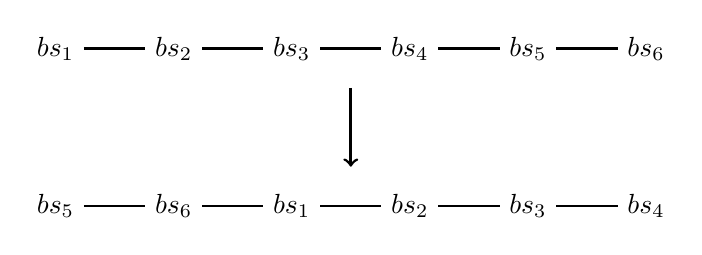
\begin{tikzpicture}
\node(1) at (0.0,0) {$bs_1$};
\node(2) at (1.5,0) {$bs_2$};
\node(3) at (3.0,0) {$bs_3$};
\node(4) at (4.5,0) {$bs_4$};
\node(5) at (6.0,0) {$bs_5$};
\node(6) at (7.5,0) {$bs_6$};

\draw[line width=1pt] (1) -- (2) -- (3) -- (4) -- (5) -- (6);

\draw[->,line width=1pt] (3.75,-0.5) -- (3.75,-1.5);

\node(1n) at (0.0,-2) {$bs_5$};
\node(2n) at (1.5,-2) {$bs_6$};
\node(3n) at (3.0,-2) {$bs_1$};
\node(4n) at (4.5,-2) {$bs_2$};
\node(5n) at (6.0,-2) {$bs_3$};
\node(6n) at (7.5,-2) {$bs_4$};

\draw[line width=1pt] (1n) -- (2n) -- (3n) -- (4n) -- (5n) -- (6n);

\end{tikzpicture}
\end{center}
\caption{Reordenamiento de una ruta con 6 paraderos, seleccionando como punto de corte la conexión entre $bs_4$ y $bs_5$.}
\label{fig:mut3}
\end{figure}
\end{enumerate}

La cantidad de veces que un clon debe ser mutado está determinado por su aptitud $x$ con respecto a la mayor aptitud $apt_{mayor}$ del conjunto de clones, la menor aptitud $apt_{menor}$ del conjunto de clones y la cantidad de rutas $n_{rutas}$ del clon. Para determinar un valor $k$, con la cantidad de veces que un clon debe ser mutado se utiliza la función $K(x)$, detallada en la Ecuación \eqref{eq:vecesmut}:

\begin{equation}
\label{eq:vecesmut}
k = \ceil*{K(x)} = \ceil*{ 1 + \frac{n_{rutas} - 1}{apt_{menor} - apt_{mayor}} (x- apt_{menor})}
\end{equation}

Dado que $x$ puede tener valores entre la aptitud menor y la aptitud mayor, $apt_{menor} \leq x \leq apt_{mayor}$. Evaluando la función $K(x)$, se tiene que $K(apt_{menor})=1$ y $k(apt_{mayor})=n_{rutas}$, por lo tanto $1 \leq K(x) \leq n_{rutas}$. En la Figura \ref{fig:k(x)} se muestra la función $K(x)$ de manera gráfica. Esta función corresponde a una recta con pendiente positiva igual a $(n_{rutas}-1)/(apt_{mayor}-apt_{menor})$. De esta forma, el clon dentro del conjunto de clones con mejor aptitud será mutado 1 vez, mientras que el clon con peor aptitud se mutará tantas veces como rutas tenga. Clones que están en puntos intermedios se mutarán más a medida que tengan mayor aptitud. La cantidad $k$ que determina la cantidad de veces que un clon se mutará utilizará esta función aproximada al entero inmediatamente superior. Con esta función se asegura la generación de diversidad de soluciones, donde todos los clones serán mutados al menos 1 vez y se mutarán más a medida que su aptitud sea mayor. Una consideración importante a destacar, para mantenerse en el terreno de las soluciones factibles, es que el operador de mutación 1 (agregar un paradero) está prohibido para rutas con el máximo de paraderos y el operador de mutación 2 (eliminar un paradero) está prohibido para rutas con el mínimo de paraderos.


\begin{figure}[!htb]
\begin{center}
\begin{tikzpicture}
\node[draw,circle,fill=black,scale=0.4](1) at (1,1) {};
\node[draw,circle,fill=black,scale=0.4](2) at (4,3) {};
\draw[->] (-0.5,0) -- (5,0) node[pos=1,above right] {$x$};
\draw[->] (0,-0.5) -- (0,4) node[pos=1,above left] {$K(x)$};
\draw[-] (1) -- (2);

\draw[-] (-0.1,1) -- (0.1,1) node[pos=0,left] {1};
\draw[-] (-0.1,3) -- (0.1,3) node[pos=0,left] {$n_{rutas}$};

\draw[-] (1,-0.1) -- (1,0.1) node[pos=0,below] {$apt_{menor}$};
\draw[-] (4,-0.1) -- (4,0.1) node[pos=0,below] {$apt_{mayor}$};

\draw[-,dotted] (1,0) -- (1) -- (0,1);
\draw[-,dotted] (4,0) -- (2) -- (0,3);

\end{tikzpicture}
\end{center}
\caption{Gráfica de la función $K(x)$}
\label{fig:k(x)}
\end{figure}

\subsection{Selección de mejores soluciones para el conjunto de memoria}

Luego de la mutación de clones, se copian hasta $mp$ de los clones a la población $P$. El tope máximo de clones a copiar está acotado superiormente por el tamaño de la población \popsize. El criterio escogido para copiar unos clones sobre otros es el ranking basado en la dominacia de pareto, mostrado en la Ecuación \eqref{eq:ranking}.

\begin{equation}
\label{eq:ranking}
rank(x_i,t) = 1+p_i^{(t)}
\end{equation}

El ranking para una solución $x_i$ con respecto a un conjunto $t$ es 1 + $p_i^{(t)}$, donde $p_i^{(t)}$ es la cantidad de soluciones que dominan a $x_{i}$ en el conjunto $t$. Los clones seleccionados para pasar al conjunto $P$ son escogidos por el valor de ranking que tengan con respecto al conjunto de clones. Los primeros clones en copiarse a la población $P$ serán aquellos con menor valor de ranking, luego se seleccionarán clones en orden ascendente hasta completar la población \popsize{} o hasta que se hayan copiado todos los clones en la población.

Los anticuerpos de la población $P$ son ordenados de acuerdo a su aptitud, luego los primeros $mm$ anticuerpos son copiados al conjunto de memoria $M$. Para determinar la cantidad $mm$ se considera la cardinalidad de la población $P$ y el parámetro \pclones{}, según la Ecuación \eqref{eq:mm}. $mm$ es aproximado al entero inmediatamente superior.

\begin{equation}
\label{eq:mm}
mm = \ceil*{|P| \cdot \pclones}
\end{equation}

Al copiar soluciones al conjunto de memoria $M$ se considera solo incluir soluciones no repetidas y no dominadas.

\subsection{Selección de soluciones para conformar nueva población}

Las peores $pp$ soluciones (las últimas del conjunto ordenado $P$) son reemplazadas con nuevas soluciones generadas aleatoriamente, de acuerdo al Algoritmo \ref{alg:inicializacion}. La cantidad $pp$ es calculada considerando la cardinalidad de la población $P$ y el parámetro \preemplazo{}, de acuerdo a la Ecuación \ref{eq:pp}. $pp$ es aproximado al entero inmediatamente superior.

\begin{equation}
\label{eq:pp}
pp = \ceil*{|P| \cdot \preemplazo}
\end{equation}

